\documentclass[11pt,a4paper]{article}

% ============================================
% PACKAGES
% ============================================
\usepackage[utf8]{inputenc}
\usepackage[T1]{fontenc}
\usepackage[english]{babel}
\usepackage{amsmath,amssymb,amsthm}
\usepackage{parskip}
\usepackage{mathtools}
\usepackage{graphicx}
\usepackage{booktabs}
\usepackage{multirow}
\usepackage[hidelinks]{hyperref}
\usepackage{xcolor}
\usepackage{enumitem}
\usepackage[margin=2.5cm]{geometry}
\usepackage{microtype}
\usepackage{caption}
\usepackage{natbib}
\usepackage{tcolorbox}
\usepackage{tikz}
\usepackage{pgfplots}
\pgfplotsset{compat=1.18}
\usetikzlibrary{shapes,arrows,positioning}
\usepackage{float}
\usepackage{url}

\usepackage{algorithm}
\usepackage{algorithmic}

% ============================================
% THEOREM ENVIRONMENTS
% ============================================
\newtheorem{theorem}{Theorem}
\newtheorem{lemma}[theorem]{Lemma}
\newtheorem{proposition}[theorem]{Proposition}
\newtheorem{corollary}[theorem]{Corollary}
\newtheorem{assumption}{Assumption}
\newtheorem{definition}{Definition}
\newtheorem{remark}{Remark}

% ============================================
% CUSTOM COMMANDS
% ============================================
\newcommand{\E}{\mathbb{E}}
\newcommand{\Var}{\text{Var}}
\newcommand{\Prob}{\mathbb{P}}
\newcommand{\logit}{\text{logit}}
\newcommand{\expit}{\text{expit}}
\newcommand{\tauQ}{\tau}
\newcommand{\tauD}{\tau^{\text{diff}}}



% ============================================
% TITLE
% ============================================
\title{
  \vspace{-1cm}
  Beyond Differences: Doubly Robust Meta-Learners\\for Ratio-Based Treatment Effects%
  \footnote{Code, data, and scripts to reproduce the experiments are available at \url{https://github.com/michaelfuchs90/ratiobasedcate}.
  }
}

\author{
  Michael Fuchs \\
  \small Munich, Germany \\
  \small \texttt{michael.fuchs@outlook.de}
}

\date{\today}

% ============================================
% DOCUMENT
% ============================================
\begin{document}

\maketitle
\begin{abstract}
When treatment decisions depend on relative lift rather than absolute
differences, the ratio-based CATE
$\tau(x) = \mathbb{E}[Y|W{=}1,X{=}x] / \mathbb{E}[Y|W{=}0,X{=}x]$ is
the appropriate estimand. Yet existing estimators either impose log-linear
parametric structure or apply generic regression without robustness
guarantees for this functional. We introduce the \emph{Q-Learner}, which
decomposes $\tau(x)$ into a product of two odds ratios, enabling direct
estimation of the ratio CATE through two propensity models without
requiring outcome regression. We further derive doubly robust
augmentations for both S/T- and Q-style ratio learners and characterize
their distinct robustness properties. In benchmarks on seven RCTs, no
single learner dominates, but the S-Learner is the most consistently
competitive method. On five observational datasets, DR-S log emerges as
the strongest method for ranking, consistent with its classical double
robustness guarantee.
\end{abstract}

\section{Introduction}
\label{sec:introduction}

Estimating heterogeneous treatment effects is central to causal inference,
with applications spanning personalized medicine, targeted marketing, and
public policy. The dominant approach estimates the \emph{difference-based}
conditional average treatment effect
\begin{equation}
\tau_{\text{diff}}(x) = \mathbb{E}[Y|W{=}1,X{=}x] - \mathbb{E}[Y|W{=}0,X{=}x],
\end{equation}
for which a rich methodological toolkit exists, including S-, T-, X-, R-,
and DR-Learners \citep{kunzel2019metalearners, nie2021quasi,
kennedy2022semiparametric}. For binary outcomes with heterogeneous
baseline rates, however, the difference-based CATE can be difficult to
interpret and unstable to estimate. A difference of
$\tau_{\text{diff}}(x) = 0.05$ represents a sixfold increase when the
baseline conversion is $\mu_0(x) = 0.01$, but merely a 25\% lift when
$\mu_0(x) = 0.2$. The ratio-based CATE
\begin{equation}
\label{eq:ratio-cate}
\tau(x) = \frac{\mathbb{E}[Y|W{=}1,X{=}x]}{\mathbb{E}[Y|W{=}0,X{=}x]}
\end{equation}
avoids this dependence on the baseline scale. When baseline rates are low
but vary widely across subgroups and treatment effects are moderate, the
ratio-based CATE is often the more natural and stable measure. Conversely,
when baseline rates are high and relatively homogeneous, the
difference-based CATE is perfectly adequate and easier to estimate. In
practice, many important application domains fall into the former regime:
clinical trials typically exhibit event rates of 1--20\%, and marketing
campaigns conversion rates of 1--10\%. Empirically, the relative scale
is often less sensitive to the baseline event rate than the absolute
scale---\citet{schmid1998} show that control-group event rates
predict absolute but not relative treatment effects across trials,
suggesting that the ratio scale better captures the intrinsic treatment
mechanism. Relative effects are also the dominant reporting format in
clinical subgroup analyses \citep{andersen2021, deeks2002}.



Despite these practical advantages, the literature on ratio-based CATE estimation
remains limited. Existing approaches either impose parametric log-linear
structure that cannot capture complex heterogeneity, or apply generic
outcome regression (S- or T-Learner style) without exploiting the
multiplicative structure of the ratio functional and without robustness
guarantees against model misspecification. 



One might attempt to recover $\tau(x)$ from existing difference-based
estimators via $\tau(x) = 1 + \tau_{\text{diff}}(x)/\mu_0(x)$, but this
requires an additional estimate of $\mu_0(x)$, and errors in both
$\hat{\tau}_{\text{diff}}$ and $\hat{\mu}_0$ compound through the
division---particularly when $\mu_0(x)$ is small, which is precisely the
regime where the ratio-based CATE is most valuable. Alternatively, one
could turn the ratio into a difference via
$\log\tau(x) = \log\mu_1(x) - \log\mu_0(x)$ and apply existing
difference-based methods on the log scale. However, this still requires
separate log-outcome models, and no doubly robust estimator for the heterogeneous ratio CATE exists in the current literature. More generally, robustness
guarantees derived for difference-based estimators do not transfer through
nonlinear transformations. Dedicated methods for the ratio functional are
therefore necessary.





\subsection{Contributions}


We address this gap with two complementary contributions. First, we
introduce the \emph{Q-Learner}, which exploits a Bayes-rule identity to
decompose the ratio CATE into a product of two odds ratios:
\begin{equation*}
\tau(x) = \frac{P(W{=}1|Y{=}1,X{=}x)}{P(W{=}0|Y{=}1,X{=}x)} \cdot
           \frac{P(W{=}0|X{=}x)}{P(W{=}1|X{=}x)}.
\end{equation*}
This reduces ratio CATE estimation to two binary classification
tasks---a propensity model and a converter-propensity model---without
requiring outcome regression. The Q-Learner directly optimizes
$\hat{\tau}(x)$ through its component classifiers, making it naturally
amenable to hyperparameter tuning and model selection. 
We further show that estimating propensity from data is
preferable to using the known propensity even in RCTs, and introduce the
Q-Simple Learner to confirm this empirically.


Second, we derive \emph{doubly robust augmentations} for both S/T-style and
Q-style ratio learners---on both direct and log scale---using influence-function-based corrections. These
augmentations eliminate first-order bias from nuisance estimation errors,
providing formal robustness guarantees. Crucially, the two constructions
exhibit \emph{different} robustness properties: DR-S/T achieves classical
double robustness (consistency if either propensity or outcome model is
correct), while DR-Q achieves only conditional robustness requiring exact
propensity knowledge---a distinction with stark empirical consequences in
observational settings. 


We evaluate all methods on seven RCT and five observational datasets (100
seeds each). In experimental settings with known propensity, no single
learner dominates, but the S-Learner proves the most consistently
competitive method in both ranking and calibration. In observational
settings, DR-S log emerges as the strongest method for ranking, confirming
the theoretical distinction between classical and conditional double
robustness.


\subsection{Related Work}
\label{sec:related}
\paragraph{Doubly Robust and Semiparametric Methods.}
Augmented inverse-probability-weighted (AIPW) estimators
\citep{robins1994estimation} provide the foundation for doubly robust
inference. \citet{bickel1993efficient} and \citet{van2000asymptotic}
establish the semiparametric efficiency theory we rely on.
\citet{chernozhukov2018double} introduced cross-fitting to remove
nuisance-estimation bias, which we adopt throughout.
\citet{foster2023orthogonal} generalise this line of work via Neyman
orthogonality, providing the theoretical foundation for loss-based and
influence-function-based learners of the kind we derive.

\paragraph{Meta-Learners for Difference-Based CATE.}
\citet{kunzel2019metalearners} introduced S-, T-, and X-Learners.
\citet{nie2021quasi} proposed the R-Learner, which directly targets
$\tau_{\text{diff}}(x)$ via a loss-based approach.
\citet{kennedy2022semiparametric} reviews doubly robust and
semiparametric methods for CATE estimation, and \citet{kennedy2023optimal}
establishes oracle rates for the DR-Learner; our DR-S/T and DR-Q
constructions adapt this pseudo-outcome paradigm to the ratio functional. These methods target
$\tau_{\text{diff}}(x)$ and do not directly apply to ratio estimation.
Our outcome-regression-based DR learners (DR-T, DR-S;
Section~\ref{sec:dr}) and DR-Q learner are ratio-specific constructions
derived from the influence function of the ratio functional.

\paragraph{Ratio-based CATE Estimation.}
Closest to our setting, \citet{yadlowsky2021ratio} propose a doubly
robust estimator for the ratio-based CATE using observational data,
combining propensity- and outcome-regression-based pseudo-outcomes
followed by arbitrary second-stage regression. Our work differs in three
ways: (i) we introduce the Q-Learner parameterisation, which reduces
ratio-CATE estimation to two classification tasks without requiring
outcome regression; (ii) we derive \emph{two distinct} DR
augmentations---DR-S/T and DR-Q---and characterise their differing
robustness properties (classical vs.\ conditional); and (iii) we
empirically benchmark both families across twelve datasets. Causal
forests \citep{athey2019grf} estimate heterogeneous effects via local
moment conditions and can in principle target non-standard functionals,
but do not provide an out-of-the-box estimator or efficiency theory for
the ratio CATE.

\paragraph{Relative Risk Estimation.}
Log-binomial and modified Poisson regression
\citep{zou2004modified, greenland2004model} estimate marginal or
conditionally linear relative risks but cannot capture nonlinear
heterogeneity. \citet{richardson2017modeling} develop a semiparametric
framework for the joint modelling of the relative risk and the risk
difference, characterising the nuisance tangent space for these
functionals. \citet{shirvaikar2023} modify causal forests to target
relative risk via GLM-based node splitting; their approach retains a
GLM-based splitting criterion and does not provide doubly robust
guarantees. \citet{boughdiri2025} derive doubly robust estimators for
the marginal risk ratio, establishing asymptotic normality and
confidence intervals; their work targets population-level effects
rather than heterogeneous CATEs. Concurrently, \citet{gao2025dina}
propose the DINA estimator (difference in natural parameters) via an
R-Learner-style extension for exponential families. For Bernoulli
outcomes DINA targets the conditional log-odds ratio; for Poisson (count)
outcomes it coincides with the conditional log risk ratio, paralleling
our log-scale variants. Their method requires choosing an outcome
family, whereas the Q-Learner identity and our DR augmentations target
the risk ratio directly without such a specification. DINA also differs
in construction: it adapts the R-Learner's Robinson-style loss via
exponential-family likelihoods, whereas our DR learners use explicit
influence-function-based pseudo-outcomes.



\paragraph{Uplift Modeling.}
The marketing literature \citep{radcliffe2011} focuses on ranking by
treatment effect. We address both ranking and calibration.

The remainder of this paper is organized as follows.
Section~\ref{sec:setup} establishes notation and assumptions.
Section~\ref{sec:q-learner} derives the Q-Learner identity.
Section~\ref{sec:dr} develops the doubly robust extensions.
Section~\ref{sec:experiments} presents the empirical evaluation, and
Section~\ref{sec:conclusion} concludes.


\section{Setup and Notation}
\label{sec:setup}

We work within the standard potential outcomes framework
\citep{rubin1974}. Each unit is characterized by a vector of pre-treatment
covariates $X \in \mathcal{X}$, a binary treatment indicator
$W \in \{0,1\}$, and a binary outcome $Y \in \{0,1\}$. 

Our target estimand is the ratio-based conditional average treatment
effect:
\begin{equation}
\tau(x) = \frac{\mu_1(x)}{\mu_0(x)},
\end{equation}
where $\mu_w(x) = P(Y{=}1 \mid W{=}w, X{=}x)$ denotes the response
surface under treatment arm $w$. The ratio $\tau(x)$ quantifies how much
more likely the outcome becomes under treatment relative to control, for
units with covariates $x$.

Identification of $\tau(x)$ from observational data requires two standard
assumptions:

\begin{assumption}[Unconfoundedness]
\label{ass:unconf}
$(Y(1), Y(0)) \perp W \mid X$
\end{assumption}

\begin{assumption}[Overlap]
\label{ass:overlap}
$0 < e(x) < 1$ for all $x \in \mathcal{X}$,
\end{assumption}
where $e(x) = P(W{=}1 \mid X{=}x)$ is the propensity score. In addition,
the ratio functional requires that the denominator is bounded away from
zero:

\begin{assumption}[Positivity of Control Response]
\label{ass:positivity}
$\mu_0(x) > 0$ for all $x \in \mathcal{X}$.
\end{assumption}

This assumption ensures that $\tau(x)$ is well-defined and is satisfied
whenever the outcome has non-negligible baseline prevalence---the typical
case in the applications we consider (conversion rates $\geq 1\%$).
In practice, regions where $\mu_0(x)$ is very small lead to unstable
estimates; we address this through clipping (Appendix~\ref{app:clipping}).

Beyond these standard quantities, the Q-Learner
(Section~\ref{sec:q-learner}) relies on two additional objects:
\begin{itemize}[leftmargin=2em]
    \item The \textbf{converter propensity}
    $p(x) = P(W{=}1 \mid Y{=}1, X{=}x)$: the probability of having been
    treated, conditional on a positive outcome.
    \item The \textbf{marginal conversion probability}
    $m(x) = P(Y{=}1 \mid X{=}x)$: the unconditional outcome rate given
    covariates.
\end{itemize}
These are observable quantities that do not require additional assumptions
beyond those stated above.

%==============================================================================
\section{The Q-Learner}
\label{sec:q-learner}
%==============================================================================

We now derive a meta-learner that directly exploits the multiplicative
structure of the ratio CATE. The key observation is the following
identification result:

Under Assumptions~\ref{ass:unconf}--\ref{ass:positivity}, for binary
outcomes $Y \in \{0,1\}$:
\begin{equation}
\label{eq:q-identity}
\tau(x) = \frac{p(x)}{1-p(x)} \cdot \frac{1-e(x)}{e(x)}
\end{equation}
where $p(x) = P(W{=}1|Y{=}1,X{=}x)$ is the treatment probability among
converters and $e(x) = P(W{=}1|X{=}x)$ is the propensity. To prove the
relation, apply Bayes' theorem to
$\mu_1(x) = P(Y{=}1|W{=}1,X{=}x)$:
\begin{equation}
\mu_1(x) = \frac{P(W{=}1|Y{=}1,X{=}x) \cdot P(Y{=}1|X{=}x)}{P(W{=}1|X{=}x)}
          = \frac{p(x) \cdot m(x)}{e(x)}
\end{equation}
Similarly, $\mu_0(x) = (1-p(x)) \cdot m(x) / (1-e(x))$. Taking the
ratio, $m(x)$ cancels:
\begin{equation}
\tau(x) = \frac{\mu_1(x)}{\mu_0(x)}
         = \frac{p(x)}{1-p(x)} \cdot \frac{1-e(x)}{e(x)}
\end{equation}

The identity has an intuitive interpretation: if treatment increases
conversion ($\tau(x) > 1$), then converters are disproportionately likely
to have been treated relative to the overall propensity, i.e.,
$p(x) > e(x)$. The ratio
$\frac{p(x)/(1-p(x))}{e(x)/(1-e(x))}$ quantifies exactly this excess on
the odds scale.

The Q-Learner Identity suggests a simple estimation strategy:
\begin{enumerate}[leftmargin=2em]
\item \textbf{Step 1:} Estimate propensity score $\hat{e}(x)$ from the
observed treatment assignments using all observations
(Section~\ref{sec:q-simple} explains why estimation is preferred even
when $e(x)$ is known)
\item \textbf{Step 2:} Estimate converter treatment probability
$\hat{p}(x)$ using only observations with $Y=1$
\item \textbf{Step 3:} Compute CATE estimate:
$\hat{\tau}(x) = \frac{\hat{p}(x)}{1-\hat{p}(x)} \cdot
\frac{1-\hat{e}(x)}{\hat{e}(x)}$
\end{enumerate}



Compared to S- and T-Learners, which estimate outcome models and derive the treatment effect indirectly, the
Q-Learner offers three structural advantages:
\begin{itemize}[leftmargin=1em]
    \item \textbf{Direct optimization of $\tau$}: Since $\hat{\tau}(x)$
    is a deterministic function of $\hat{p}(x)$ and $\hat{e}(x)$,
    hyperparameter tuning of the component models directly improves the
    treatment effect estimate. In contrast, the S-Learner optimizes the
    outcome model $\hat{\mu}(x,w)$, and improvements in outcome
    prediction do not necessarily translate to better treatment effect
    estimation. This makes the Q-Learner particularly amenable to
    automated model selection (Section~\ref{sec:experiments}).
    \item \textbf{Balanced classification}: In A/B tests with
    $e(x) \approx 0.5$ and low conversion rates, the Q-Learner transforms
    a highly imbalanced outcome regression problem into a balanced
    classification problem among converters.
    \item \textbf{Flexibility}: Any probabilistic classifier can serve as
    base model for both stages.
\end{itemize}

\begin{remark}[Single Model via Offset]
\label{rem:single-model}
Taking logs of \eqref{eq:q-identity} one arrives at
\begin{equation}
    \log\tau(x) = \logit(p(x)) - \logit(e(x)).
\end{equation}
This suggests fitting a single logistic regression for $p(x)$ with
$\logit(\hat{e}(x))$ as offset:
\begin{equation}
\logit(p(x)) = \logit(\hat{e}(x)) + f(x)
\end{equation}
where $f(x)$ models the treatment effect heterogeneity. The fitted model
directly yields $\hat{\tau}(x) = \exp(\hat{f}(x))$, reducing the
two-stage procedure to a single model after propensity estimation.
\end{remark}

\begin{remark}[Extension to Multi-Class Treatments]
The Q-Learner can be generalized to non-binary treatments by using
multi-class classification for $p(w, x) = P(W{=}w|Y{=}1, X{=}x)$ and
$e(w, x) = P(W{=}w|X{=}x)$:
\begin{equation}
    \tau(x, w_1, w_2) = \frac{p(w_1, x)}{p(w_2, x)} \cdot
    \frac{e(w_2, x)}{e(w_1, x)}
\end{equation}
Extensions to non-binary outcomes are possible but less straightforward;
we leave their investigation to future work.
\end{remark}

\subsection{Propensity Estimation and the Q-Simple Learner}
\label{sec:q-simple}

In RCT settings where propensity is exactly known, one might be tempted
to skip fitting a propensity model and use the known $e(x)$ directly in
the Q-Learner identity~\eqref{eq:q-identity}. This reduces CATE
estimation to a single model for $p(x)$, estimated only among
converters. This is a computationally attractive simplification, especially for
large datasets.

However, estimating propensity from data can reduce finite-sample
variance. The key insight is that $\hat{p}(x)$ and $\hat{e}(x)$ are
correlated through the same realized treatment assignments: if a
covariate region happens to contain more treated units than expected,
both $\hat{e}(x)$ and $\hat{p}(x)$ increase, and the biases partially
cancel in the product
$\frac{\hat{p}}{1-\hat{p}} \cdot \frac{1-\hat{e}}{\hat{e}}$. Using the
known $e(x)$ breaks this correlation, potentially increasing
finite-sample variance.

This variance reduction diminishes with sample size: as $n$ grows, the
realized propensity concentrates around its true value, and the
correlation benefit vanishes. For large datasets, the computational
savings from skipping propensity estimation may therefore outweigh the
small variance cost.

\paragraph{The Q-Simple Learner.}
To empirically quantify this trade-off, we introduce the \emph{Q-Simple
Learner}: a variant that uses the known propensity $e(x)$ directly in
the Q-Learner identity~\eqref{eq:q-identity}, without estimating it from
data. For RCTs with constant propensity (e.g., $e = 0.5$), this simply
means plugging in the design constant. The Q-Simple Learner is only
applicable to experimental settings where $e(x)$ is known by design.

Section~\ref{sec:experiments} confirms that Q-Learner outperforms
Q-Simple on average ($+0.015$ mean Qini), though the advantage is
concentrated on a single dataset (Lenta: $+0.087$); on the remaining six
RCTs the difference is negligible ($+0.003$). For large datasets where
computational efficiency matters, Q-Simple remains a competitive choice.


%==============================================================================
\section{Doubly Robust Extensions}
\label{sec:dr}
The Q-Learner and the naive ratio estimator $\hat{\mu}_1(x)/\hat{\mu}_0(x)$
(T-Learner) are plug-in estimators: they combine estimated nuisance
functions into $\hat{\tau}(x)$ without correction for estimation error. If any nuisance model is misspecified,
the resulting bias propagates directly into the CATE estimate.

Following the framework of \citet{kennedy2022semiparametric}, we derive
\emph{augmented} estimators that eliminate the leading-order bias through
influence-function-based corrections. Concretely, for an estimand
$\tau(x)$ that depends on nuisance functions $g$ (propensity, outcome
models, etc.), the augmented pseudo-outcome takes the form
\begin{equation}
\Gamma = \hat{\tau}(x) + \hat{\phi}_{\tau}(W, Y, X; x),
\end{equation}
where $\hat{\phi}_{\tau}$ is the estimated influence function of $\tau$
evaluated at the nuisance estimates. This correction removes the
first-order (linear) bias term, leaving a remainder of order
$O_p(\|\hat{g} - g\|_2^2)$---a product of nuisance estimation errors
that vanishes faster than any individual error alone. The resulting
estimators are \emph{oracle-efficient} in the sense of
\citet{kennedy2022semiparametric} when nuisance estimates converge at
sufficiently fast rates: regressing the pseudo-outcome $\Gamma$ on $X$
then achieves the same convergence rate as if the true nuisance functions
were known.

The ratio CATE $\tau(x) = \mu_1(x)/\mu_0(x)$ admits two natural
parameterizations---through outcome models $(\mu_1, \mu_0)$ or through
the Q-Learner reparameterization $(p, e)$---leading to two distinct
augmented estimators. As we show below, these exhibit fundamentally
different robustness properties: DR-S/T achieves classical double robustness,
while DR-Q achieves only conditional robustness requiring exact propensity
knowledge.

\subsection{DR-S/T: Augmenting the Ratio via Outcome Models}
\label{sec:dr-t}

The T-Learner estimates $\mu_1(x)$ and $\mu_0(x)$ separately while the S-Learner includes the treatment as covariable $\mu_w(x) = \mu(w, x)$. In both cases, the ratio-based CATE can directly be evaluated $\hat{\tau}(x) = \hat{\mu}_1(x)/\hat{\mu}_0(x)$. The following augmentation can therefore be used for S- and T-Learner. The
standard AIPW influence functions for the response surfaces are:
\begin{align}
\phi_{\mu_1}(W, Y, X; x) &= \frac{W(Y - \mu_1(x))}{e(x)}, \\
\phi_{\mu_0}(W, Y, X; x) &= \frac{(1-W)(Y - \mu_0(x))}{1-e(x)}.
\end{align}
Applying the quotient rule
$\phi_{\tau} = (\phi_{\mu_1} - \tau \cdot \phi_{\mu_0})/\mu_0$ and
substituting nuisance estimates yields the DR-S/T pseudo-outcome:
\begin{equation}
\label{eq:dr-t}
\Gamma^{\text{DR-S/T}} = \hat{\tau}(X)
  + \frac{W(Y - \hat{\mu}_1(X))}{\hat{e}(X) \cdot \hat{\mu}_0(X)}
  - \frac{\hat{\tau}(X)(1-W)(Y - \hat{\mu}_0(X))}{(1-\hat{e}(X)) \cdot \hat{\mu}_0(X)}
\end{equation}
where $\hat{\tau}(X) = \hat{\mu}_1(X)/\hat{\mu}_0(X)$. The first
correction term adjusts for bias in $\hat{\mu}_1$, the second for bias
in $\hat{\mu}_0$, both weighted by the inverse propensity.




\subsubsection{Double Robustness of DR-S/T}
\label{res:dr-t-direct}


The DR-S/T estimator achieves \emph{classical double robustness}: it is
consistent for $\tau(x)$ if either
\begin{enumerate}[leftmargin=2em]
    \item[(a)] the propensity model is correct: $\hat{e}(x) = e(x)$, or
    \item[(b)] the outcome models are correct: $\hat{\mu}_0(x) = \mu_0(x)$
    and $\hat{\mu}_1(x) = \mu_1(x)$.
\end{enumerate}
We now verify both cases. Writing $\Gamma^{\text{DR-S/T}} = A + B - C$ with
$A = \hat{\tau}$,
$B = W(Y - \hat{\mu}_1)/(\hat{e}\hat{\mu}_0)$, and
$C = \hat{\tau}(1-W)(Y - \hat{\mu}_0)/((1-\hat{e})\hat{\mu}_0)$:

\begin{itemize}
\item \textbf{Case (a): $\hat{e} = e$ (correct propensity).}

Taking conditional expectations given $X = x$:
\begin{align}
\E[B \mid X{=}x] &= \frac{\mu_1(x) - \hat{\mu}_1(x)}{\hat{\mu}_0(x)}, \\
\E[C \mid X{=}x] &= \frac{\hat{\tau}(x)(\mu_0(x) - \hat{\mu}_0(x))}{\hat{\mu}_0(x)}.
\end{align}
A first-order Taylor expansion of $\tau = \mu_1/\mu_0$ around
$(\hat{\mu}_1, \hat{\mu}_0)$ gives:
\begin{equation}
\tau(x) = \hat{\tau}(x) + \frac{\mu_1(x) - \hat{\mu}_1(x)}{\hat{\mu}_0(x)}
  - \frac{\hat{\tau}(x)(\mu_0(x) - \hat{\mu}_0(x))}{\hat{\mu}_0(x)}
  + O_p(\|\hat{\mu} - \mu\|_2^2)
\end{equation}
Therefore
$\E[\Gamma^{\text{DR-S/T}} \mid X{=}x] = \tau(x) + O_p(\|\hat{\mu} - \mu\|_2^2)$.

\item \textbf{Case (b): $\hat{\mu}_0 = \mu_0$, $\hat{\mu}_1 = \mu_1$
(correct outcome models).}

Then $A = \tau(x)$, and $\E[B \mid X{=}x] = \E[C \mid X{=}x] = 0$ since
$Y - \mu_w(X)$ has conditional mean zero given $(W, X)$. Thus
$\E[\Gamma^{\text{DR-S/T}} \mid X{=}x] = \tau(x)$ exactly, regardless of
the propensity estimate.
\end{itemize}

When both models are misspecified, the bias is
$O_p(\|\hat{e} - e\|_2 \cdot \|\hat{\mu} - \mu\|_2)$, second-order in
the nuisance estimation errors.



\subsubsection{DR-S/T on Log Scale}
\label{sec:log-scale}

When treatment effects span a wide range, direct-scale pseudo-outcomes
exhibit heteroscedastic variance proportional to the effect magnitude. A
log-scale formulation provides variance stabilization. Since
$\log \tau(x) = \log \mu_1(x) - \log \mu_0(x)$ and the influence
functions for $\log \mu_w$ are $\phi_{\log \mu_w} = \phi_{\mu_w}/\mu_w$,
we obtain:
\begin{equation}
\label{eq:dr-t-log}
\Gamma^{\text{DR-S/T}}_{\log} = \log \hat{\mu}_1(X) - \log \hat{\mu}_0(X)
  + \frac{W(Y - \hat{\mu}_1(X))}{\hat{e}(X) \hat{\mu}_1(X)}
  - \frac{(1-W)(Y - \hat{\mu}_0(X))}{(1-\hat{e}(X)) \hat{\mu}_0(X)}
\end{equation}
The log-scale DR-S/T inherits the same double robustness property as the
direct-scale version.


\subsection{DR-Q: Augmenting the Q-Learner}
\label{sec:dr-q}


While DR-S/T achieves classical double robustness, the Q-Learner parameterization leads to a weaker robustness structure,
as we now show. The Q-Learner identity~\eqref{eq:q-identity} expresses $\tau(x)$ as a product:
\begin{equation}
\tau(x) = \underbrace{\frac{p(x)}{1-p(x)}}_{A(x)} \cdot \underbrace{\frac{1-e(x)}{e(x)}}_{B(x)}
\end{equation}


We apply the product rule $\phi_\tau = B\phi_A + A\phi_B$. For $A(x) =
p(x)/(1-p(x))$, the influence function on the converter subpopulation,
lifted to the full population via $m(x)$, is
$\phi_A = Y(W-p(x))/(m(x)(1-p(x))^2)$. For $B(x) = (1-e(x))/e(x)$,
the influence function is $\phi_B = -(W-e(x))/e(x)^2$. Substituting
nuisance estimates yields the DR-Q pseudo-outcome:
\begin{equation}
\label{eq:dr-q}
\Gamma^{\text{DR-Q}} = \hat{\tau}(X) + \frac{(1-\hat{e}(X)) \cdot Y(W-\hat{p}(X))}{\hat{e}(X) \cdot \hat{m}(X)(1-\hat{p}(X))^2} - \frac{\hat{p}(X)(W-\hat{e}(X))}{(1-\hat{p}(X))\hat{e}(X)^2}
\end{equation}

where $\hat{\tau}(X) = \frac{\hat{p}(X)}{1-\hat{p}(X)} \cdot \frac{1-\hat{e}(X)}{\hat{e}(X)}$ is the plug-in Q-Learner estimate. Since both parameterizations target the same functional $\tau(x)$, the
augmentation terms are algebraically equivalent to those of
DR-S/T~\eqref{eq:dr-t} after substitution of the identities
$\mu_1 = pm/e$ and $\mu_0 = (1-p)m/(1-e)$.



\subsubsection{Conditional Robustness of DR-Q}
\label{res:dr-q-direct}

Unlike DR-S/T, the DR-Q estimator does \emph{not} achieve classical double robustness. The reason is that the propensity score $e(x)$ appears in \emph{both} the plug-in estimate and the augmentation terms.


Concretely, the DR-Q estimator requires \emph{exact} specification of the propensity score $e(x)$. Given $\hat{e}(x) = e(x)$ \textbf{exactly}, the estimator is consistent for $\tau(x)$ if either:
\begin{enumerate}[leftmargin=2em]
    \item[(a)] the marginal conversion model is correct: $\hat{m}(x) = m(x)$, or
    \item[(b)] the converter propensity model is correct: $\hat{p}(x) = p(x)$
\end{enumerate}
If $\hat{e}(x) \neq e(x)$, the estimator is generally inconsistent regardless of the quality of $\hat{m}$ and $\hat{p}$. 

We verify both cases. Writing
\begin{equation}
    \Gamma^{\text{DR-Q}} = \underbrace{\hat{A}\hat{B}}_{\text{plug-in}} + \underbrace{\hat{B} \cdot \hat{\phi}_A}_{\text{$p$-correction}} + \underbrace{\hat{A} \cdot \hat{\phi}_B}_{\text{$e$-correction}}
\end{equation}
where $\hat{A} = \hat{p}/(1-\hat{p})$, $\hat{B} = (1-\hat{e})/\hat{e}$, and $\hat{\phi}_A$, $\hat{\phi}_B$ are the estimated influence function contributions.

\begin{itemize}
    \item 

\textbf{Case (a): $\hat{e} = e$ and $\hat{m} = m$ (correct propensity and marginal conversion).}

With correct propensity, $\hat{B} = B$ and $\E[\hat{\phi}_B \mid X] = 0$.
For the $p$-correction term, note that
$\E[Y(W - \hat{p}(X)) \mid X{=}x] = m(x)(p(x) - \hat{p}(x))$, so with
$\hat{m} = m$ the marginal conversion cancels:
\begin{equation}
\E[\hat{B} \cdot \hat{\phi}_A \mid X{=}x] = B(x) \cdot
\frac{p(x) - \hat{p}(x)}{(1-\hat{p}(x))^2}
\end{equation}
Using a first-order Taylor expansion of $A = p/(1-p)$ around $\hat{p}$:
\begin{equation}
A(x) = \hat{A}(x) + \frac{p(x) - \hat{p}(x)}{(1-\hat{p}(x))^2} + O_p(\|\hat{p} - p\|_2^2)
\end{equation}

Therefore:
\begin{equation}
\E[\Gamma^{\text{DR-Q}} \mid X{=}x] = \hat{A}(x)B(x) + B(x)\frac{p(x) - \hat{p}(x)}{(1-\hat{p}(x))^2} = \tau(x) + O_p(\|\hat{p} - p\|_2^2)
\end{equation}
\item \textbf{Case (b): $\hat{e} = e$ and $\hat{p} = p$ (correct propensity and converter propensity).}


Then $\hat{A} = A$, $\hat{B} = B$, so the plug-in equals $\tau(x)$. Both correction terms have conditional mean zero: $\E[\hat{\phi}_A \mid X] = 0$ since $W - p(X)$ has mean zero given $(Y{=}1, X)$, and $\E[\hat{\phi}_B \mid X] = 0$ since $W - e(X)$ has mean zero given $X$. Thus $\E[\Gamma^{\text{DR-Q}} \mid X{=}x] = \tau(x)$ exactly.
\end{itemize}



\subsubsection{DR-Q on Log Scale}
Taking logarithms of the Q-Learner identity gives $\log \tau(x) = \logit(p(x)) - \logit(e(x))$, where $\logit(u) = \log(u/(1-u))$. Applying the delta method with $\frac{d}{dp}\logit(p) = 1/(p(1-p))$:
\begin{equation}
\label{eq:dr-q-log}
\Gamma^{\text{DR-Q}}_{\log} = \underbrace{\logit(\hat{p}(X)) - \logit(\hat{e}(X))}_{\text{plug-in}} + \underbrace{\frac{Y(W-\hat{p}(X))}{\hat{m}(X) \hat{p}(X)(1-\hat{p}(X))}}_{\text{correction for } p} - \underbrace{\frac{W-\hat{e}(X)}{\hat{e}(X)(1-\hat{e}(X))}}_{\text{correction for } e}
\end{equation}

The log-scale DR-Q has the same conditional robustness properties as the direct-scale version (Section~\ref{res:dr-q-direct}). 

\subsubsection{DR-Q-Simple Learner}
\label{sec:dr-q-simple}

The conditional robustness of DR-Q demands $\hat{e}(x) = e(x)$. Under
this requirement, the $e$-augmentation term has conditional expectation
zero and provides no bias correction. Analogous to the Q-Simple Learner (Section~\ref{sec:q-simple}) this motivates a simplified
construction that operates only on converters ($Y=1$) and eliminates the
need to estimate $m(x)$:
\begin{equation}
\label{eq:dr-q-simple}
\Gamma^{\text{DR-Q-Simple}} = \hat{\tau}(X) +
\frac{(1-e(X)) \cdot (W-\hat{p}(X))}{e(X) \cdot (1-\hat{p}(X))^2}
\end{equation}
where $\hat{\tau}(X) = \frac{\hat{p}(X)}{1-\hat{p}(X)} \cdot
\frac{1-e(X)}{e(X)}$ and $e(x)$ is the known propensity. Given exact
$e(x)$:
\begin{equation}
\mathbb{E}[\Gamma^{\text{DR-Q-Simple}} \mid X=x, Y=1] = \tau(x) +
O_p(\|\hat{p} - p\|_2^2)
\end{equation}
The DR-Q-Simple learner is particularly attractive for RCT applications:
it eliminates the need to estimate $m(x)$, operates only on the
$n_1 = \sum_i Y_i$ converters, and requires only a single nuisance
function $\hat{p}(x)$. The simplification comes at a cost in asymptotic
efficiency.


\subsubsection{DR-Q-Simple on Log Scale}
\label{sec:dr-q-simple-log}

Applying the same log-scale construction as in DR-Q
(Section~\ref{sec:log-scale}) but restricting to converters and using
known $e(x)$:
\begin{equation}
\label{eq:dr-q-simple-log}
\Gamma^{\text{DR-Q-Simple}}_{\log} = \underbrace{\logit(\hat{p}(X)) -
\logit(e(X))}_{\text{plug-in}} +
\underbrace{\frac{W-\hat{p}(X)}{\hat{p}(X)(1-\hat{p}(X))}}_{\text{correction for } p}
\end{equation}
This pseudo-outcome is computed only for observations with $Y=1$ and
inherits the same robustness property: consistency for $\log\tau(x)$
with bias $O_p(\|\hat{p} - p\|_2^2)$.




\subsection{Choosing the Appropriate Learner}
\label{sec:choosing}

The theoretical properties derived above directly inform the choice of
estimator for a given application setting.

\paragraph{Observational studies.}
When propensity must be estimated from data, outcome-regression-based DR
learners (DR-T, DR-S) are the only viable choices. DR-Q's conditional
robustness requires exact propensity knowledge, which is unavailable in
observational settings; misspecification of $e(x)$ renders DR-Q
inconsistent regardless of the quality of other nuisance models
(Section~\ref{res:dr-q-direct}). DR-T and DR-S, by contrast, remain
consistent if either the propensity or the outcome models are correct
(Section~\ref{res:dr-t-direct}). Between the two, DR-S uses a joint
outcome model that provides additional regularization, which can be
beneficial on smaller datasets.

\paragraph{Randomized experiments.}
When propensity is known by design, both DR-S/T and DR-Q families are
applicable. DR-Q-Simple (Section~\ref{sec:dr-q-simple}) is the most
parsimonious option: it requires only a single nuisance model
$\hat{p}(x)$, operates only on converters, and avoids estimation of both
$e(x)$ and $m(x)$. For large datasets, this computational advantage is
particularly relevant, and the variance cost from using known rather than
estimated propensity becomes negligible (Section~\ref{sec:q-simple}). The
full DR-Q may provide efficiency gains through
the additional augmentation term.


\paragraph{Log-scale variants.}
When treatment effects vary over a wide range, log-scale formulations
provide natural variance stabilization: the pseudo-outcomes
$\Gamma_{\log}$ have approximately homoscedastic variance regardless of
effect magnitude, whereas direct-scale pseudo-outcomes exhibit variance
that grows with the effect size.

\paragraph{Plug-in vs.\ DR learners.}
DR augmentation introduces additional variance through the correction
terms. When nuisance models are well-specified (e.g., in large RCTs with
simple structure), plug-in methods (Q-Learner, S-Learner) are expected to achieve
better calibration at the cost of robustness. The choice therefore
depends on whether the practitioner prioritizes robustness against
misspecification or calibration accuracy.

Section~\ref{sec:experiments} confirms these theoretical predictions
empirically and provides quantitative guidance.



\section{Empirical Evaluation}
\label{sec:experiments}

We now systematically evaluate which learner performs best under which
conditions, with the goal of providing practitioners with concrete
guidance on method selection. In particular, we test whether the
theoretical expectations from Section~\ref{sec:choosing} hold in
practice: whether DR-S/T outperforms DR-Q in observational settings (as
predicted by the distinction between classical and conditional
robustness), and whether estimating propensity from data outperforms
using known propensity (Q-Learner vs.\ Q-Simple).


\subsection{Setup}

We evaluate thirteen learners: six plug-in methods (S, T, Q, Q-Simple and X) and seven doubly robust variants (DR-T, DR-T log,
DR-S, DR-S log, DR-Q, DR-Q log, and DR-Q-Simple for RCTs). Q-Simple and
DR-Q-Simple are only applicable to RCT datasets where propensity is known
by design; observational benchmarks use ten learners.

\paragraph{Datasets.}
We select datasets to cover a range of sample sizes ($n = 1.6$k--$1.4$M),
conversion rates (0.9\%--68\%), and treatment fractions (18\%--85\%).
Crucially, we separate RCT datasets, where propensity is known by
design, from observational datasets, where propensity must be estimated
and confounding is present. This separation reflects the fundamentally
different estimation challenges and allows us to test the theoretical
distinction between classical and conditional double robustness.

\begin{table}[h]
\centering
\caption{RCT benchmark datasets. Propensity $e(x)$ is known by design.
$^*$Semi-synthetic: both potential outcomes observed, treatment simulated
with $e=0.5$.}
\label{tab:datasets-rct}
\setlength{\tabcolsep}{6pt}
\begin{tabular}{lrrrl}
\hline
Dataset & $n$ & Conv.\ & Treat.\ & Domain \\
\hline
Criteo \citep{diemert2018}              & 1{,}398k &  4.7\% & 85.0\% & E-commerce \\
Hillstrom (Visit) \citep{hillstrom2008} &  64k     & 14.7\% & 66.8\% & Email \\
Hillstrom (Conv.) \citep{hillstrom2008} &  64k     &  0.9\% & 66.8\% & Email \\
MegaFon \citep{megafon2019}             & 600k     & 20.4\% & 50.1\% & Telecom \\
X5 Retail \citep{x5retail2020}          & 200k     & 62.0\% & 49.9\% & Retail \\
Lenta \citep{lenta2021}                 & 687k     &  5.9\% & 50.0\% & Grocery \\
Twins$^*$ \citep{louizos2017}           &  71k     &  3.6\% & 50.0\% & Neonatal \\
\hline
\end{tabular}
\end{table}

\begin{table}[h]
\centering
\caption{Observational benchmark datasets. Propensity $e(x)$ must be
estimated.}
\label{tab:datasets-obs}
\setlength{\tabcolsep}{6pt}
\begin{tabular}{lrrrl}
\hline
Dataset & $n$ & Conv.\ & Treat.\ & Domain \\
\hline
LaLonde \citep{lalonde1986}      &  2.7k & 60.0\% & 36.6\% & Job training \\
RHC \citep{connors1996rhc}       &  5.7k & 68.5\% & 38.0\% & Medical \\
Cattaneo \citep{cattaneo2010}    &  4.6k &  6.0\% & 18.6\% & Birthweight \\
NHEFS \citep{hernan2020}         &  1.6k & 19.5\% & 26.3\% & Smoking \\
JTPA \citep{abadie2002}          &  9.2k & 50.0\% & 44.0\% & Job training \\
\hline
\end{tabular}
\end{table}



\paragraph{Metrics.}
We evaluate two complementary metrics. The \emph{Qini coefficient}
measures ranking quality: how well a learner identifies individuals with
the highest treatment effect. We adapt the normalized Qini
coefficient~\citep{radcliffe2011} to ratio-based effects by integrating
the ratio rather than the difference:
\[
  \mathrm{Qini}_\text{ratio} = \int_0^1 \frac{\hat{Y}^{(1)}(s)}
  {\hat{Y}^{(0)}(s)} \, \mathrm{d}s - \frac{Y^{(1)}}{Y^{(0)}},
\]
where $\hat{Y}^{(w)}(s)$ is the mean outcome in arm $w$ among the
top-$s$ fraction ranked by predicted $\hat{\tau}(x)$. Higher is better.

The \emph{multiplicative calibration error} measures how accurately
predicted effect sizes match realized effects. We compute the error on
the log scale, where over- and under-prediction are treated
symmetrically ($\log(0.8) = -\log(1.25)$), then exponentiate to obtain
an interpretable multiplicative factor:
\begin{equation}
\label{eq:cal-error}
\mathrm{CalError} = \exp\left(\frac{\sum_{b=1}^{B} n_b \,\bigl|\log
\bar{\hat{\tau}}_b - \log \hat{\tau}_b^{\mathrm{emp}}\bigr|}
{\sum_{b=1}^{B} n_b}\right),
\end{equation}
where $\bar{\hat{\tau}}_b$ is the mean predicted effect in bin $b$ and
$\hat{\tau}_b^{\mathrm{emp}} = \bar{Y}_b^{(1)}/\bar{Y}_b^{(0)}$ is the
empirical ratio within that bin ($B = 10$ equal-frequency bins). A
CalError of $1.0\times$ indicates perfect calibration; $1.5\times$ means
predictions are on average off by a factor of 1.5.

\paragraph{Comparison across datasets.}
Since absolute Qini values vary by orders of magnitude across datasets
(e.g., MegaFon $\approx 1.3$ vs.\ Lenta $\approx 0.02$), we summarize
learner performance using the \emph{gap to the best learner} per dataset:
\begin{equation}
\label{eq:qini-gap}
\Delta Q_{l,d} = Q_{l,d} - \max_{l'} Q_{l',d}.
\end{equation}
This quantity is always $\leq 0$, with $0$ indicating the best learner on
that dataset. Averaging $\Delta Q_{l,d}$ across datasets yields the mean
Qini gap: how many Qini points a learner loses on average relative to the
dataset-specific optimum. Analogously, for calibration we compute the gap
to the best-calibrated learner:
$\Delta C_{l,d} = \mathrm{CalError}_{l,d} - \min_{l'} \mathrm{CalError}_{l',d}$
(always $\geq 0$, with $0$ indicating best calibration). These
normalized metrics allow fair comparison across datasets of different
difficulty; full per-dataset results are in
Appendix~\ref{app:sec:full-results}.




\paragraph{Implementation.}
All methods use LightGBM \citep{lightgbm} for nuisance and final-stage
models with default hyperparameters. DR learners use 5-fold cross-fitting
\citep{chernozhukov2018double} to generate out-of-fold nuisance
predictions. Final-stage regressors use a Poisson objective to enforce
$\hat{\tau}(x) > 0$. To improve stability, we clip nuisance estimates and pseudo-outcomes as described in Appendix~\ref{app:clipping}. Results are averaged over 100 random seeds
per dataset, with each seed determining the train/test split.

\subsection{Ranking Analysis}
\label{sec:ranking}

We evaluate which learners most consistently achieve near-optimal ranking
performance across datasets. Figure~\ref{fig:qini-gap} summarizes the
results using the gap-to-best metric~\eqref{eq:qini-gap}: learners
closer to zero with lower variance are more reliably competitive.

\begin{figure}[t]
\centering
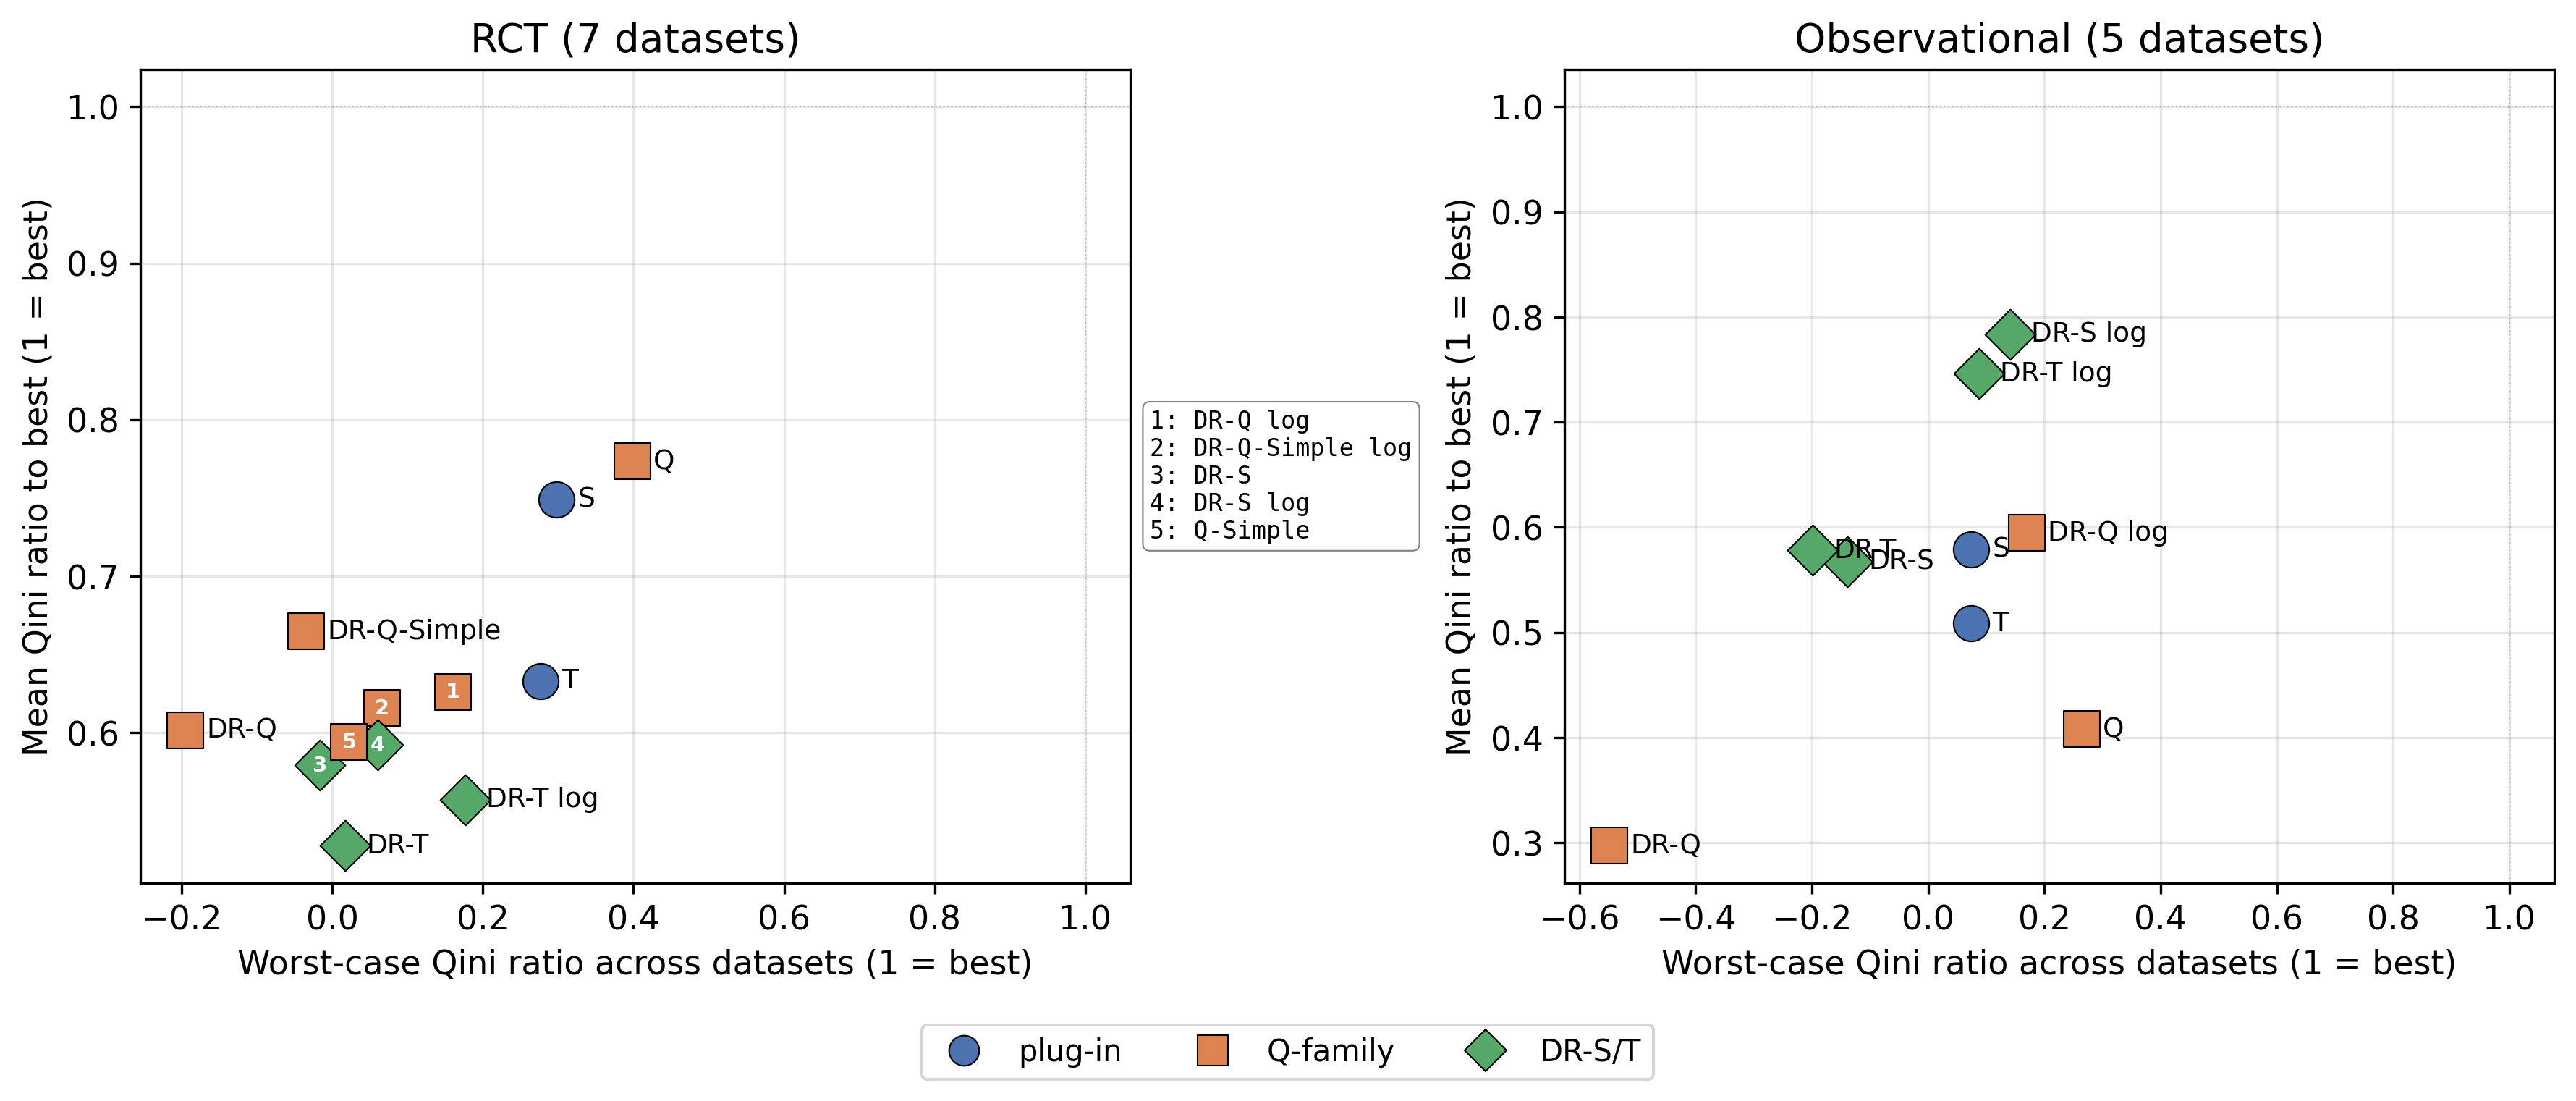
\includegraphics[width=\textwidth]{fig_qini_gap.png}
\caption{Mean Qini gap to the best learner per dataset ($0$ = best) vs.\
cross-dataset standard deviation, for RCT (left) and observational
(right) datasets. The ideal learner sits in the upper-right corner
(small gap, low variance).}
\label{fig:qini-gap}
\end{figure}

\subsubsection{RCT Datasets}

Table~\ref{tab:results-rct} (Appendix~\ref{app:sec:full-results}) reports
per-dataset Qini coefficients on the seven RCT datasets.
\textbf{No single learner dominates}: seven datasets produce six
different winners (DR-S, DR-Q-Simple, DR-Q, T-Learner, Q-Learner, and
X-Learner). The S-Learner never achieves the highest Qini on any
individual dataset, yet it is the most \emph{consistently competitive}
method: its mean gap to the best learner is only $-0.091$ Qini points
with the lowest cross-dataset standard deviation ($0.091$), meaning it
is reliably close to optimal regardless of the dataset
(Figure~\ref{fig:qini-gap}, left panel).

By contrast, learners that win on individual datasets exhibit higher
variance: DR-Q (mean gap $-0.099$, std $0.120$), DR-Q-Simple ($-0.101$,
std $0.135$), and the T-Learner ($-0.133$, std $0.159$) can be the best
on one dataset but substantially worse on another. The DR-S/T family
performs weakest on RCT data (mean gap $-0.14$ to $-0.20$), suggesting
that outcome-regression-based DR augmentation provides limited benefit
when propensity is known and datasets are large.

\paragraph{Q-Learner vs.\ Q-Simple.}
The Q-Learner (mean gap $-0.111$) slightly outperforms Q-Simple
($-0.126$), but the advantage is almost entirely driven by a single
dataset (Lenta: $+0.087$). On the remaining six datasets, the difference
is negligible. Q-Simple remains competitive, particularly for large
datasets where its computational simplicity is attractive.

\paragraph{Practical recommendation.}
For practitioners seeking reliably good performance without extensive
model comparison, the S-Learner is the safest default on RCT data. For
practitioners willing to evaluate multiple candidates, the Q-family and
DR-Q-family offer the potential for higher Qini on specific datasets.


\subsubsection{Observational Datasets}

Table~\ref{tab:results-obs} (Appendix~\ref{app:sec:full-results}) reveals
a strikingly different picture on observational data, where propensity
must be estimated. \textbf{DR-S log is the clear winner}: its mean gap to
the best learner is only $-0.019$ Qini points with a standard deviation
of $0.028$---meaning it is nearly always the best or within a negligible
margin of the best on every dataset. DR-T log is a solid second (mean gap
$-0.059$, std $0.076$), followed by a large drop to DR-Q log ($-0.103$)
and the plug-in learners (S: $-0.106$, T: $-0.117$).

This confirms the theoretical prediction from
Section~\ref{sec:choosing}: outcome-regression-based DR learners with
classical double robustness (DR-S/T) clearly outperform both plug-in
methods and DR-Q in observational settings. The advantage of DR-S over
DR-T (both in log and direct scale) reflects the regularization benefit
of joint outcome modeling, which yields more stable $\hat{\mu}_1$ and
$\hat{\mu}_0$ estimates on the smaller observational datasets
($n = 1.6$k--$9.2$k).

\paragraph{Collapse of DR-Q.}
The most striking result is the failure of DR-Q (mean gap $-0.250$, std
$0.242$): it produces \emph{negative} Qini on both RHC ($-0.106$) and
NHEFS ($-0.082$), meaning worse-than-random targeting. This directly
confirms that DR-Q's conditional robustness requires exact propensity
knowledge (Section~\ref{res:dr-q-direct}), which is unavailable in
observational settings. DR-Q log (mean gap $-0.103$) fares substantially
better due to variance stabilization, but still lags behind DR-S/T log.

\paragraph{Log vs.\ direct scale.}
Across all DR learners, log-scale variants consistently outperform their
direct-scale counterparts on observational data (DR-S log: $-0.019$ vs.\
DR-S: $-0.171$; DR-T log: $-0.059$ vs.\ DR-T: $-0.160$). The
variance-stabilizing reparametrization is particularly beneficial on
smaller datasets where direct-scale pseudo-outcomes can produce extreme
values.

\paragraph{Practical recommendation.}
For observational settings, \textbf{DR-S log is the recommended default},
combining classical double robustness with joint-model regularization and
log-scale variance stabilization. DR-T log is a viable alternative when
the practitioner prefers separate outcome models per treatment arm.


\subsection{Calibration Analysis}
\label{sec:calibration}

Direct-scale DR pseudo-outcomes introduce systematic scale bias. We
apply a rank-preserving log-linear recalibration
($\log\hat{\tau}_{\mathrm{cal}} = \hat{a} + \hat{b}\log\hat{\tau}$,
fit on bin-level means), which reduces calibration error for direct-scale
DR learners (DR-Q: $-27\%$, DR-T: $-22\%$, DR-S: $-10\%$) but worsens
it for log-scale DR and plug-in methods
(Table~\ref{tab:calibration}, Appendix~\ref{app:sec:full-results}).

\begin{figure}[t]
\centering
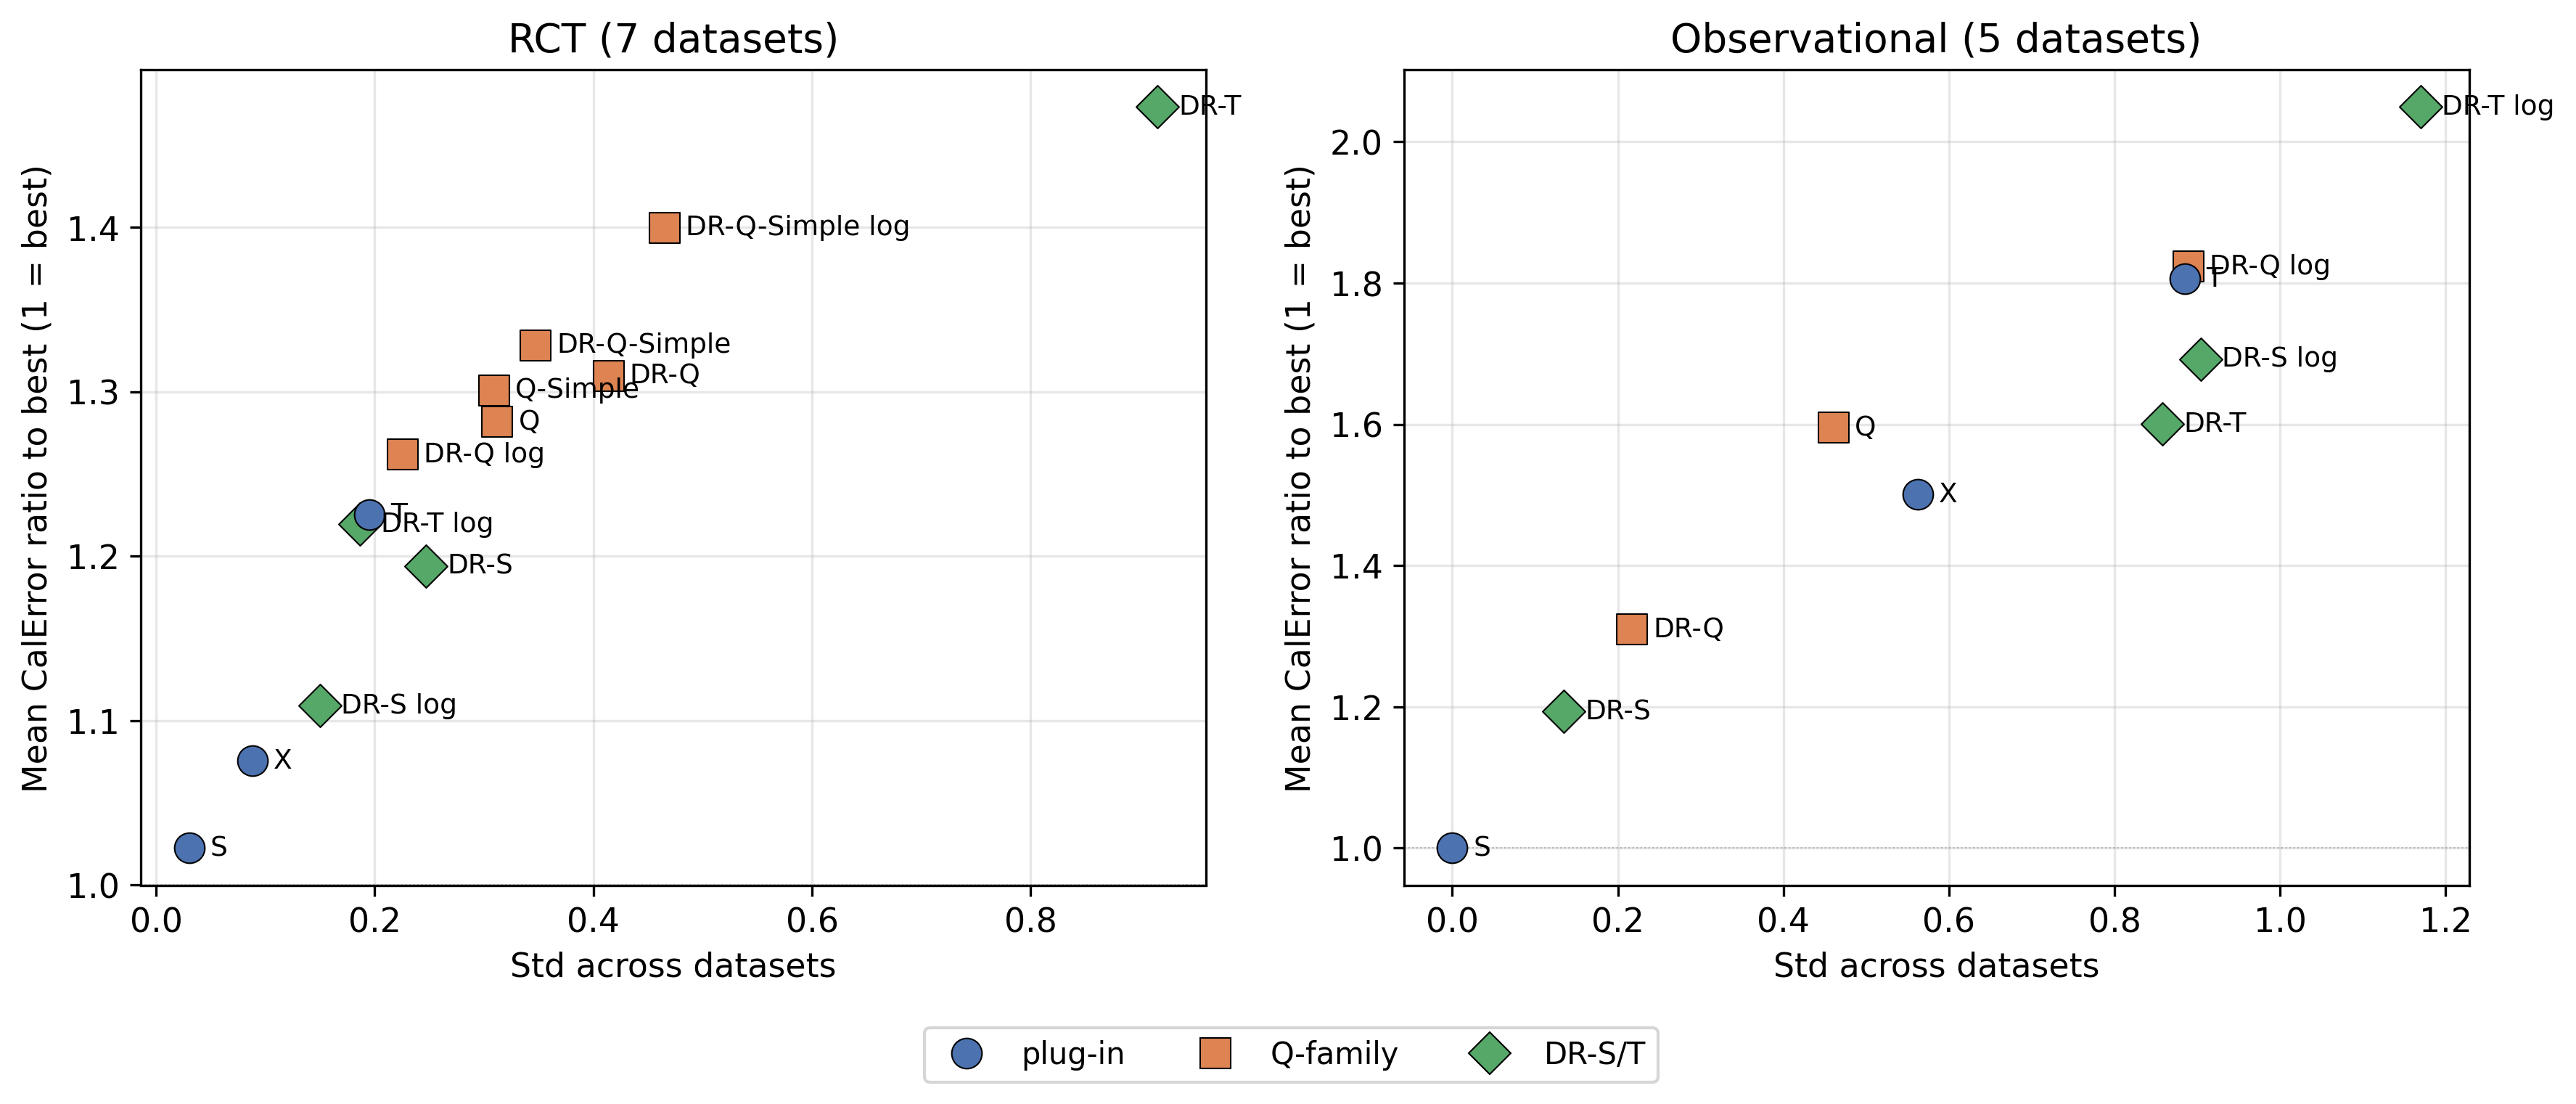
\includegraphics[width=\textwidth]{fig_cal_gap.png}
\caption{Mean calibration gap to the best-calibrated learner per dataset
($0$ = best) vs.\ cross-dataset standard deviation, for RCT (left) and
observational (right) datasets. Each learner at its best calibration
configuration. The ideal learner sits at the origin.}
\label{fig:cal-gap}
\end{figure}

Figure~\ref{fig:cal-gap} shows the calibration gap across datasets. On
RCT data, the \textbf{S-Learner} dominates calibration (mean gap $0.038$,
std $0.064$), followed distantly by X-Learner ($0.126$) and DR-S log
($0.127$). DR learners on direct scale remain poorly calibrated even
after recalibration. On observational data, the pattern is similar: the
S-Learner provides the most reliable calibration, while DR methods
trade calibration accuracy for ranking robustness.


\subsection{Summary}

\begin{enumerate}
    \item \textbf{RCTs: S-Learner is the safe default and mandatory when
    calibration matters.} On RCT data, no single learner achieves the
    best Qini on all datasets (seven datasets produce six different
    winners). However, the S-Learner is the most \emph{consistently
    competitive} method: it has the smallest mean Qini gap to the best
    ($-0.091$) with the lowest variance ($0.091$), and simultaneously
    the best calibration (gap $0.038$). For practitioners seeking
    reliably good performance, the S-Learner suffices. For practitioners
    seeking the absolute best ranking on a specific dataset, multiple
    candidates (particularly the DR-Q family) should be evaluated. We
    note that the S-Learner's consistency advantage may partly reflect
    default hyperparameters that favor outcome prediction; with
    learner-specific tuning, the Q-Learner's results may improve more
    than the S-Learner's, since the ratio-based CATE is directly
    optimized through its component classifiers.

    \item \textbf{Observational: DR-S log dominates ranking; S-Learner
    dominates calibration.} In observational settings, DR-S log is nearly
    always the best ranker or within negligible margin (mean Qini gap
    $-0.019$, std $0.028$). DR-T log is a solid alternative ($-0.059$).
    The advantage of DR methods over plug-in learners (S: $-0.106$,
    T: $-0.117$) confirms that doubly robust augmentation provides
    genuine value when propensity must be estimated. DR-Q collapses under
    confounding (gap $-0.250$), validating the theoretical distinction
    between classical and conditional double robustness. As on RCT data,
    the S-Learner remains by far the best-calibrated method.

    \item \textbf{Estimating propensity beats knowing it---by a slight
    margin.} Q-Learner outperforms Q-Simple by $+0.015$ mean Qini on
    RCTs, driven almost entirely by Lenta ($+0.087$). Q-Simple remains
    competitive for large datasets.

    \item \textbf{Log-scale variants dominate direct-scale.} Across all
    DR learners and both settings, log-scale variants consistently
    outperform their direct-scale counterparts (e.g., DR-S log gap
    $-0.019$ vs.\ DR-S $-0.171$ on observational data). The
    variance-stabilizing reparametrization is particularly beneficial on
    smaller datasets. Post-hoc recalibration partially mitigates the
    scale bias of direct-scale DR ($-10\%$ to $-27\%$) but should not be
    applied to log-scale or plug-in methods.
\end{enumerate}

\paragraph{Limitations.}
Our evaluation uses binary outcomes, a single base learner (LightGBM with
default hyperparameters), and fixed clipping thresholds. Results may
differ with learner-specific hyperparameter tuning, other model classes,
or continuous outcomes. The observational datasets are small
($n = 1.6$k--$9.2$k), limiting the precision of comparisons. Without
access to true CATEs, we evaluate ranking and calibration but cannot
assess pointwise estimation accuracy.


\section{Conclusion}
\label{sec:conclusion}

We introduced the Q-Learner, a meta-learner for ratio-based CATEs that
decomposes $\tau(x)$ into a product of odds ratios via a Bayes-rule
identity, reducing estimation to two binary classification tasks that
directly optimize the treatment effect estimate. We derived doubly robust
augmentations for both outcome-regression-based (DR-S/T) and
Q-Learner-based (DR-Q) ratio estimators, and characterized their distinct
robustness properties: classical double robustness for DR-S/T versus
conditional robustness for DR-Q.

Our benchmark across twelve datasets and 100 seeds per dataset reveals a
clear practical picture. In RCT settings with known propensity, modern
gradient boosting models already estimate outcome surfaces well on the
typically large datasets, making the S-Learner the safest choice. While
never the single best ranker on any dataset, it is consistently very
close to optimal in ranking and consistently the best in calibration.
Only when best-in-class ranking is required should other methods be
evaluated---and since no single learner dominates, all candidates must be
tested. In observational settings, the picture changes: DR-S log emerges
as the clear winner for ranking (mean Qini gap to best: $-0.019$),
combining classical double robustness with the regularization of joint
outcome modeling and log-scale variance stabilization. DR-Q's conditional
robustness proves insufficient under confounding, producing
worse-than-random targeting on strongly confounded datasets. For
calibration, the S-Learner dominates also on observational data.


These results suggest a simple decision rule: use the S-Learner when
calibration matters or as a reliable default on RCTs; use DR-S log when
ranking is the primary objective in observational settings. The Q-Learner
remains independently valuable for settings where direct optimizability
of $\hat{\tau}(x)$ matters---since hyperparameter tuning of its component
classifiers directly improves the treatment effect estimate, it is
particularly suited for automated model selection pipelines.

Several directions remain open. Extending the framework to continuous and
time-to-event outcomes would broaden applicability. Investigating whether
the S-Learner's consistency advantage persists under learner-specific
hyperparameter tuning---particularly for the Q-Learner, whose component
classifiers directly optimize $\hat{\tau}(x)$---is an important practical
question. Developing confidence intervals for ratio-based CATEs, building
on the influence functions derived here, would enable formal inference.
Finally, adaptive procedures for learner selection based on dataset
characteristics could automate the practitioner's choice among the
methods developed in this paper.

\paragraph{Code and data availability.}
All code, dataset loaders, and scripts to reproduce the experiments in
this paper are available at
\url{https://github.com/michaelfuchs90/ratiobasedcate}.
The repository includes the 33{,}000-row benchmark CSV, the notebook that
generates all figures and tables, and a README with replication
instructions.

\paragraph{Acknowledgements.}
I thank Kristina Weidner and Marco Breitig for reading through the
manuscript and providing valuable feedback, and Dominik Krei\ss{} for
stimulating conversations about the topic.

%==============================================================================
% REFERENCES
%==============================================================================
\bibliographystyle{plainnat}
\begin{thebibliography}{99}

\bibitem[Abadie et~al.(2002)]{abadie2002}
Abadie, A., Angrist, J., and Imbens, G. (2002).
Instrumental variables estimates of the effect of subsidized training on the quantiles of trainee earnings.
\emph{Econometrica}, 70(1):91--117.

\bibitem[Bickel et~al.(1993)]{bickel1993efficient}
Bickel, P.~J., Klaassen, C.~A., Ritov, Y., and Wellner, J.~A. (1993).
\emph{Efficient and Adaptive Estimation for Semiparametric Models}. Springer.

\bibitem[Cattaneo(2010)]{cattaneo2010}
Cattaneo, M.~D. (2010).
Efficient semiparametric estimation of multi-valued treatment effects under ignorability.
\emph{Journal of Econometrics}, 155(2):138--154.

\bibitem[Chernozhukov et~al.(2018)]{chernozhukov2018double}
Chernozhukov, V., Chetverikov, D., Demirer, M., Duflo, E., Hansen, C., Newey, W., and Robins, J. (2018).
Double/debiased machine learning for treatment and structural parameters.
\emph{The Econometrics Journal}, 21(1):C1--C68.

\bibitem[Connors et~al.(1996)]{connors1996rhc}
Connors, A.~F., Speroff, T., Dawson, N.~V., et~al. (1996).
The effectiveness of right heart catheterization in the initial care of critically ill patients.
\emph{JAMA}, 276(11):889--897.

\bibitem[Diemert et~al.(2018)]{diemert2018}
Diemert, E., Betlei, A., Renaudin, C., and Amini, M.~R. (2018).
A large scale benchmark for uplift modeling.
\emph{Proceedings of AdKDD \& TargetAd, KDD}.

\bibitem[Boughdiri et~al.(2025)]{boughdiri2025}
Boughdiri, A., Josse, J., and Scornet, E. (2025).
Quantifying treatment effects: Estimating risk ratios via observational studies.
\emph{Proceedings of the 42nd International Conference on Machine Learning (ICML)}.


\bibitem[Hern{\'a}n and Robins(2020)]{hernan2020}
Hern{\'a}n, M.~A. and Robins, J.~M. (2020).
\emph{Causal Inference: What If}.
Chapman \& Hall/CRC.

\bibitem[Hillstrom(2008)]{hillstrom2008}
Hillstrom, K. (2008).
The MineThatData E-Mail Analytics And Data Mining Challenge.
\emph{MineThatData Blog}.

\bibitem[Ke et~al.(2017)]{lightgbm}
Ke, G., Meng, Q., Finley, T., Wang, T., Chen, W., Ma, W., Ye, Q., and Liu, T.~Y. (2017).
LightGBM: A highly efficient gradient boosting decision tree.
\emph{NeurIPS}, 30.

\bibitem[Kennedy(2022)]{kennedy2022semiparametric}
Kennedy, E.~H. (2022).
Semiparametric doubly robust targeted double machine learning: a review.
\emph{arXiv:2203.06469}.

\bibitem[K{\"u}nzel et~al.(2019)]{kunzel2019metalearners}
K{\"u}nzel, S.~R., Sekhon, J.~S., Bickel, P.~J., and Yu, B. (2019).
Metalearners for estimating heterogeneous treatment effects using machine learning.
\emph{PNAS}, 116(10):4156--4165.

\bibitem[LaLonde(1986)]{lalonde1986}
LaLonde, R.~J. (1986).
Evaluating the econometric evaluations of training programs with experimental data.
\emph{The American Economic Review}, 76(4):604--620.

\bibitem[Lenta(2021)]{lenta2021}
Lenta Uplift Modeling Dataset (2021).
\url{https://sklift.readthedocs.io/en/latest/datasets.html}.

\bibitem[Louizos et~al.(2017)]{louizos2017}
Louizos, C., Shalit, U., Mooij, J.~M., Sontag, D., Zemel, R., and Welling, M. (2017).
Causal effect inference with deep latent-variable models.
\emph{NeurIPS}, 30.

\bibitem[MegaFon(2019)]{megafon2019}
MegaFon Uplift Competition (2019).
\emph{Open Data Science Community}.

\bibitem[Nie and Wager(2021)]{nie2021quasi}
Nie, X. and Wager, S. (2021).
Quasi-oracle estimation of heterogeneous treatment effects.
\emph{Biometrika}, 108(2):299--319.

\bibitem[Robins et~al.(1994)]{robins1994estimation}
Robins, J.~M., Rotnitzky, A., and Zhao, L.~P. (1994).
Estimation of regression coefficients when some regressors are not always observed.
\emph{Journal of the American Statistical Association}, 89(427):846--866.

\bibitem[Radcliffe and Surry(2011)]{radcliffe2011}
Radcliffe, N.~J. and Surry, P.~D. (2011).
Real-world uplift modelling with significance-based uplift trees.
\emph{White Paper, Stochastic Solutions}.

\bibitem[Rubin(1974)]{rubin1974}
Rubin, D.~B. (1974).
Estimating causal effects of treatments in randomized and nonrandomized studies.
\emph{Journal of Educational Psychology}, 66(5):688--701.

\bibitem[van~der~Vaart(2000)]{van2000asymptotic}
van~der~Vaart, A.~W. (2000).
\emph{Asymptotic Statistics}. Cambridge University Press.

\bibitem[X5 Retail(2020)]{x5retail2020}
X5 Retail Hero Uplift Competition (2020).
\url{https://retailhero.ai/}.

\bibitem[Zou(2004)]{zou2004modified}
Zou, G. (2004).
A modified Poisson regression approach to prospective studies with binary data.
\emph{American Journal of Epidemiology}, 159(7):702--706.



\bibitem[Andersen(2021)]{andersen2021}
Andersen, L.~W. (2021).
Absolute vs.\ relative effects---implications for subgroup analyses.
\emph{Trials}, 22(1):50.

\bibitem[Athey et~al.(2019)]{athey2019grf}
Athey, S., Tibshirani, J., and Wager, S. (2019).
Generalized random forests.
\emph{The Annals of Statistics}, 47(2):1148--1178.

\bibitem[Deeks(2002)]{deeks2002}
Deeks, J.~J. (2002).
Issues in the selection of a summary statistic for meta-analysis of clinical trials with binary outcomes.
\emph{Statistics in Medicine}, 21(11):1575--1600.

\bibitem[Gao and Hastie(2025)]{gao2025dina}
Gao, Z. and Hastie, T. (2025).
Estimating heterogeneous treatment effects for general responses.
\emph{Biometrics}, 81(4):ujaf162.

\bibitem[Schmid et~al.(1998)]{schmid1998}
Schmid, C.~H., Lau, J., McIntosh, M.~W., and Cappelleri, J.~C. (1998).
An empirical study of the effect of the control rate as a predictor of treatment efficacy in meta-analysis of clinical trials.
\emph{Statistics in Medicine}, 17(17):1923--1942.

\bibitem[Shirvaikar et~al.(2023)]{shirvaikar2023}
Shirvaikar, V., Stor{\aa}s, A., Lin, X., and Holmes, C. (2023).
Targeting relative risk heterogeneity with causal forests.
\emph{arXiv preprint arXiv:2309.15793}.

\bibitem[Foster and Syrgkanis(2023)]{foster2023orthogonal}
Foster, D.~J. and Syrgkanis, V. (2023).
Orthogonal statistical learning.
\emph{Annals of Statistics}, 51(3). arXiv:1901.09036.

\bibitem[Greenland(2004)]{greenland2004model}
Greenland, S. (2004).
Model-based estimation of relative risks and other epidemiologic measures in studies of common outcomes and in case-control studies.
\emph{American Journal of Epidemiology}, 160(4):301--305.

\bibitem[Kennedy(2023)]{kennedy2023optimal}
Kennedy, E.~H. (2023).
Towards optimal doubly robust estimation of heterogeneous causal effects.
\emph{Electronic Journal of Statistics}, 17(2). arXiv:2004.14497.

\bibitem[Richardson et~al.(2017)]{richardson2017modeling}
Richardson, T.~S., Robins, J.~M., and Wang, L. (2017).
On modeling and estimation for the relative risk and risk difference.
\emph{Journal of the American Statistical Association}, 112(519):1121--1130.

\bibitem[Yadlowsky et~al.(2020)]{yadlowsky2021ratio}
Yadlowsky, S., Pellegrini, F., Lionetto, F., Braune, S., and Tian, L. (2020).
Estimation and validation of ratio-based conditional average treatment effects using observational data.
\emph{arXiv preprint arXiv:1912.06977}.


\end{thebibliography}

%==============================================================================
% APPENDIX
%==============================================================================
\appendix

\section{Full Benchmark Results}
\label{app:sec:full-results}

\subsection{Qini on RCT Datasets}
\begin{table}[H]
\centering
\footnotesize
\caption{Qini coefficient on RCT datasets (mean over 100 seeds; SE in parentheses). Best per column in \textbf{bold}. Bottom row: mean across all learners per dataset.}
\label{tab:results-rct}
\setlength{\tabcolsep}{3pt}
\begin{tabular}{l | rrrrrrr | r r}
\hline
Learner & H(Vis) & H(Conv) & Criteo & MegaFon & X5 & Lenta & Twins & $\bar{Q}$ & $\sigma_D$ \\
\hline
S-Learner
 & 0.435 & 0.371 & 0.334 & 1.424 & 0.073 & 0.027 & 0.087 & \textbf{0.393} & 0.483 \\
 & \scriptsize(0.016) & \scriptsize(0.065) & \scriptsize(0.007) & \scriptsize(0.005) & \scriptsize(0.001) & \scriptsize(0.005) & \scriptsize(0.006) & & \\[2pt]
T-Learner
 & 0.321 & 0.181 & 0.263 & \textbf{1.533} & 0.055 & 0.025 & 0.076 & 0.351 & 0.533 \\
 & \scriptsize(0.015) & \scriptsize(0.049) & \scriptsize(0.007) & \scriptsize(0.005) & \scriptsize(0.001) & \scriptsize(0.004) & \scriptsize(0.008) & & \\[2pt]
Q-Learner
 & 0.219 & 0.507 & 0.454 & 1.228 & 0.030 & \textbf{0.089} & 0.086 & 0.373 & 0.420 \\
 & \scriptsize(0.012) & \scriptsize(0.053) & \scriptsize(0.009) & \scriptsize(0.004) & \scriptsize(0.001) & \scriptsize(0.004) & \scriptsize(0.008) & & \\[2pt]
Q-Simple
 & 0.215 & 0.516 & 0.427 & 1.236 & 0.025 & 0.002 & 0.083 & 0.358 & 0.435 \\
 & \scriptsize(0.012) & \scriptsize(0.051) & \scriptsize(0.007) & \scriptsize(0.004) & \scriptsize(0.001) & \scriptsize(0.003) & \scriptsize(0.008) & & \\[2pt]
X-Learner
 & 0.408 & 0.150 & 0.351 & 1.295 & 0.069 & 0.043 & \textbf{0.093} & 0.344 & 0.443 \\
 & \scriptsize(0.018) & \scriptsize(0.045) & \scriptsize(0.008) & \scriptsize(0.004) & \scriptsize(0.001) & \scriptsize(0.005) & \scriptsize(0.007) & & \\[2pt]
\hline
DR-Q
 & 0.356 & 0.580 & \textbf{0.508} & 1.184 & 0.070 & $-$0.017 & 0.013 & 0.385 & 0.426 \\
 & \scriptsize(0.016) & \scriptsize(0.055) & \scriptsize(0.009) & \scriptsize(0.004) & \scriptsize(0.001) & \scriptsize(0.005) & \scriptsize(0.009) & & \\[2pt]
DR-Q log
 & 0.268 & 0.514 & 0.193 & 1.263 & 0.058 & 0.014 & 0.085 & 0.342 & 0.440 \\
 & \scriptsize(0.015) & \scriptsize(0.054) & \scriptsize(0.004) & \scriptsize(0.004) & \scriptsize(0.001) & \scriptsize(0.003) & \scriptsize(0.006) & & \\[2pt]
DR-Q-Simple
 & 0.336 & \textbf{0.615} & 0.461 & 1.145 & 0.043 & $-$0.003 & 0.080 & 0.383 & 0.408 \\
 & \scriptsize(0.015) & \scriptsize(0.061) & \scriptsize(0.009) & \scriptsize(0.004) & \scriptsize(0.001) & \scriptsize(0.003) & \scriptsize(0.006) & & \\[2pt]
DR-Q-Simple log
 & 0.243 & 0.600 & 0.449 & 1.229 & 0.026 & 0.006 & 0.073 & 0.375 & 0.438 \\
 & \scriptsize(0.014) & \scriptsize(0.049) & \scriptsize(0.008) & \scriptsize(0.004) & \scriptsize(0.001) & \scriptsize(0.003) & \scriptsize(0.011) & & \\[2pt]
DR-T
 & 0.438 & 0.010 & 0.331 & 1.236 & 0.075 & 0.016 & 0.003 & 0.301 & 0.447 \\
 & \scriptsize(0.017) & \scriptsize(0.035) & \scriptsize(0.008) & \scriptsize(0.004) & \scriptsize(0.001) & \scriptsize(0.005) & \scriptsize(0.010) & & \\[2pt]
DR-T log
 & 0.319 & 0.109 & 0.157 & 1.253 & 0.059 & 0.016 & 0.092 & 0.286 & 0.437 \\
 & \scriptsize(0.014) & \scriptsize(0.040) & \scriptsize(0.003) & \scriptsize(0.004) & \scriptsize(0.001) & \scriptsize(0.004) & \scriptsize(0.006) & & \\[2pt]
DR-S
 & \textbf{0.473} & 0.321 & 0.343 & 1.195 & \textbf{0.076} & 0.004 & $-$0.002 & 0.344 & 0.418 \\
 & \scriptsize(0.017) & \scriptsize(0.053) & \scriptsize(0.007) & \scriptsize(0.004) & \scriptsize(0.002) & \scriptsize(0.005) & \scriptsize(0.010) & & \\[2pt]
DR-S log
 & 0.330 & 0.361 & 0.102 & 1.259 & 0.058 & 0.005 & 0.091 & 0.315 & 0.438 \\
 & \scriptsize(0.015) & \scriptsize(0.060) & \scriptsize(0.002) & \scriptsize(0.004) & \scriptsize(0.001) & \scriptsize(0.003) & \scriptsize(0.006) & & \\
\hline
\textit{Dataset mean} & 0.336 & 0.372 & 0.337 & 1.268 & 0.055 & 0.017 & 0.066 & & \\
\hline
\end{tabular}
\end{table}


\subsection{Qini on Observational Datasets}
\begin{table}[H]
\centering
\footnotesize
\caption{Qini coefficient on observational datasets (mean over 100 seeds; SE in parentheses). Best per column in \textbf{bold}. Bottom row: mean across all learners per dataset.}
\label{tab:results-obs}
\setlength{\tabcolsep}{3pt}
\begin{tabular}{l | rrrrr | r r}
\hline
Learner & LaLonde & RHC & Cattaneo & NHEFS & JTPA & $\bar{Q}$ & $\sigma_D$ \\
\hline
S-Learner
 & 0.153 & 0.014 & 1.124 & 0.132 & 0.032 & 0.291 & 0.470 \\
 & \scriptsize(0.022) & \scriptsize(0.005) & \scriptsize(0.096) & \scriptsize(0.047) & \scriptsize(0.006) & & \\[2pt]
T-Learner
 & 0.146 & 0.014 & 1.098 & 0.129 & 0.013 & 0.280 & 0.462 \\
 & \scriptsize(0.020) & \scriptsize(0.005) & \scriptsize(0.098) & \scriptsize(0.048) & \scriptsize(0.006) & & \\[2pt]
Q-Learner
 & 0.083 & 0.061 & 0.637 & 0.111 & 0.019 & 0.182 & 0.256 \\
 & \scriptsize(0.019) & \scriptsize(0.008) & \scriptsize(0.107) & \scriptsize(0.041) & \scriptsize(0.006) & & \\[2pt]
X-Learner
 & 0.115 & 0.014 & 1.113 & 0.005 & 0.026 & 0.255 & 0.482 \\
 & \scriptsize(0.019) & \scriptsize(0.005) & \scriptsize(0.115) & \scriptsize(0.038) & \scriptsize(0.007) & & \\[2pt]
\hline
DR-Q
 & 0.124 & $-$0.106 & 0.726 & $-$0.082 & \textbf{0.071} & 0.147 & 0.338 \\
 & \scriptsize(0.019) & \scriptsize(0.011) & \scriptsize(0.091) & \scriptsize(0.043) & \scriptsize(0.008) & & \\[2pt]
DR-Q log
 & 0.101 & 0.087 & 1.040 & 0.229 & 0.012 & 0.294 & 0.424 \\
 & \scriptsize(0.022) & \scriptsize(0.014) & \scriptsize(0.115) & \scriptsize(0.045) & \scriptsize(0.006) & & \\[2pt]
DR-T
 & \textbf{0.154} & 0.098 & 0.922 & $-$0.050 & 0.063 & 0.237 & 0.390 \\
 & \scriptsize(0.023) & \scriptsize(0.011) & \scriptsize(0.099) & \scriptsize(0.038) & \scriptsize(0.008) & & \\[2pt]
DR-T log
 & 0.133 & 0.193 & 1.126 & 0.234 & 0.006 & 0.338 & 0.449 \\
 & \scriptsize(0.022) & \scriptsize(0.015) & \scriptsize(0.099) & \scriptsize(0.036) & \scriptsize(0.006) & & \\[2pt]
DR-S
 & 0.133 & 0.098 & 0.866 & $-$0.035 & 0.067 & 0.226 & 0.363 \\
 & \scriptsize(0.021) & \scriptsize(0.011) & \scriptsize(0.081) & \scriptsize(0.035) & \scriptsize(0.008) & & \\[2pt]
DR-S log
 & 0.120 & \textbf{0.193} & \textbf{1.313} & \textbf{0.253} & 0.010 & \textbf{0.378} & 0.531 \\
 & \scriptsize(0.022) & \scriptsize(0.015) & \scriptsize(0.108) & \scriptsize(0.041) & \scriptsize(0.006) & & \\
\hline
\textit{Dataset mean} & 0.126 & 0.067 & 0.997 & 0.093 & 0.032 & & \\
\hline
\end{tabular}
\end{table}

\subsection{Calibration}
\begin{table}[H]
\centering
\caption{Effect of post-hoc log-linear recalibration. DR-Q-Simple and Q-Simple: 7 RCT datasets only. Calibration is rank-preserving: $\Delta$\,Qini $= 0$.}
\label{tab:calibration}
\setlength{\tabcolsep}{6pt}
\begin{tabular}{lrrr}
\hline
Learner & CalError (base) & CalError (cal.) & $\Delta$ \\
\hline
DR-Q & 2.70$\times$ & 1.97$\times$ & $-$27\% \\
DR-Q log & 2.42$\times$ & 3.00$\times$ & $+$24\% \\
DR-Q-Simple & 2.30$\times$ & 2.11$\times$ & $-$8\% \\
DR-Q-Simple log & 1.95$\times$ & 3.28$\times$ & $+$68\% \\
DR-T & 3.17$\times$ & 2.48$\times$ & $-$22\% \\
DR-T log & 2.42$\times$ & 3.35$\times$ & $+$38\% \\
DR-S & 2.16$\times$ & 1.95$\times$ & $-$10\% \\
DR-S log & 2.01$\times$ & 2.73$\times$ & $+$36\% \\
\hline
S-Learner & 1.47$\times$ & 2.06$\times$ & $+$40\% \\
T-Learner & 2.24$\times$ & 4.86$\times$ & $+$117\% \\
Q-Learner & 2.12$\times$ & 3.67$\times$ & $+$73\% \\
Q-Simple & 1.77$\times$ & 3.83$\times$ & $+$116\% \\
X-Learner & 1.89$\times$ & 2.80$\times$ & $+$48\% \\
\hline
\end{tabular}
\end{table}


\section{Numerical Stability through Clipping}
\label{app:clipping}
For numerical stability, we recommend the following clipping bounds as good starting points:
\begin{itemize}[leftmargin=1em]
    \item \textbf{Propensity scores}: Clip $\hat{e}(x)$ to $[\epsilon_e, 1-\epsilon_e]$ with $\epsilon_e = 0.01$
    \item \textbf{Outcome probabilities}: Clip $\hat{\mu}_w(x)$ to $[\epsilon_\mu, 1-\epsilon_\mu]$ with $\epsilon_\mu = 0.001$
    \item \textbf{Marginal conversion}: Clip $\hat{m}(x)$ to $[\epsilon_m, 1]$ with $\epsilon_m = 0.001$
    \item \textbf{Converter propensity}: Clip $\hat{p}(x)$ to $[\epsilon_p, 1-\epsilon_p]$ with $\epsilon_p = 0.01$
    \item \textbf{Pseudo-outcomes}: Clip $\Gamma^{\text{DR}}$ to $[\epsilon_\tau, 1/\epsilon_\tau]$ with $\epsilon_\tau = 0.01$
    \item \textbf{Log-scale pseudo-outcomes}: Clip $\Gamma^{\text{DR}}_{\log}$ to $[-C, C]$ with $C = 10$
\end{itemize}
While these can serve as a good starting point, in practice we recommend treating the clipping parameters as hyperparameters subject to optimization.




\end{document}


